\documentclass[options]{article}
\usepackage[]{url}
\usepackage{graphicx}
\usepackage{hyperref}
\usepackage{mathtools}

\begin{document}
\title{Simulation of two interacting squirmers}
\author{Robin and Justine}
\date{May, 2024}
\maketitle

\section{Context}
Our project is part of the ANR project NEMO, Control of Magnetic Micro-swimmers in Complex and Confined Environments.
Currently, a team of researchers is developing numerical methods to control a micro-swimmer in the arteries
of the human body.
The Squirmer model simulates bacteria with cilia by imposing boundary conditions.
Ultimately, the goal of these robots is to treat cancer cells.

\vspace{0.5cm}
\section{Objectives}
Our goal is to model the dynamics of two interacting squirmers, influenced by hydrodynamic \cite{Brumley} and collision forces.\\
We will start by reformulating the formulas of all present forces and torques.\cite{Brumley}\cite{Lauga}\\
In addition we will implement this model to realize numerical experiments. The aim of these experiments is: 
\begin{itemize}
    \item To Investigate the effects of varying the distance between the squirmers to observe
    potential modifications in their behaviors.
    \item To explore the impact of altering the parameter $\beta$, which defines the
    type of squirmers (pusher, puller, neutral swimmer), on their interactions.
    \item To conduct a comparative analysis of the interaction between a squirming micro-robot and a 
    boundary of the fluid domain. This analysis will involve varying the initial angle of the micro-robot, the distance between the swimmer and the wall, as well as the parameter $\beta$, 
    to comprehensively understand their influence on the system dynamics.
\end{itemize}

\newpage
\section{Roadmap}
\begin{center}
    \href{https://github.com/orgs/master-csmi/projects/23/views/2}{Roadmap}
    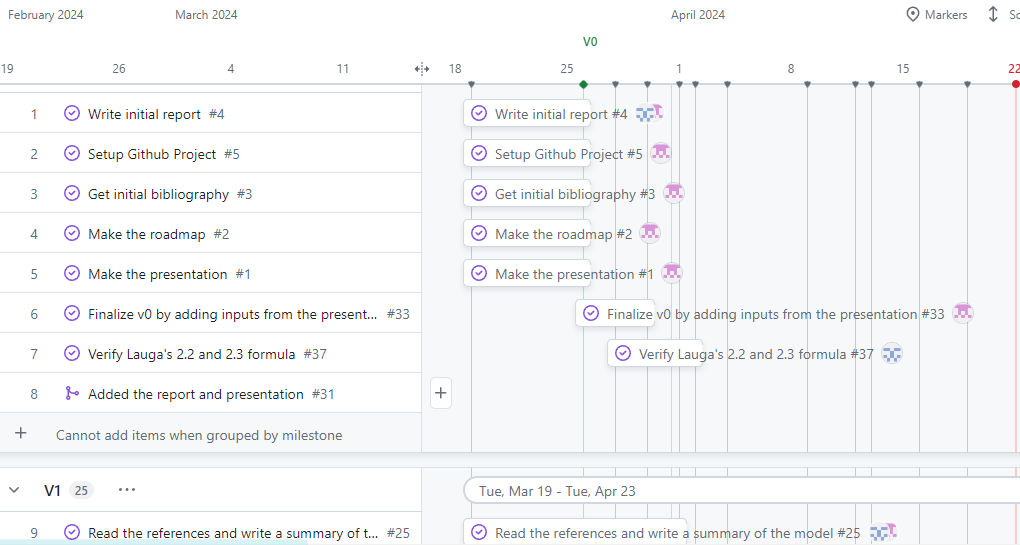
\includegraphics[width=0.9\textwidth]{Presentation/V0/images/roadmapV0_1.png}
    \vspace{1em} % Ajoute un espace vertical
    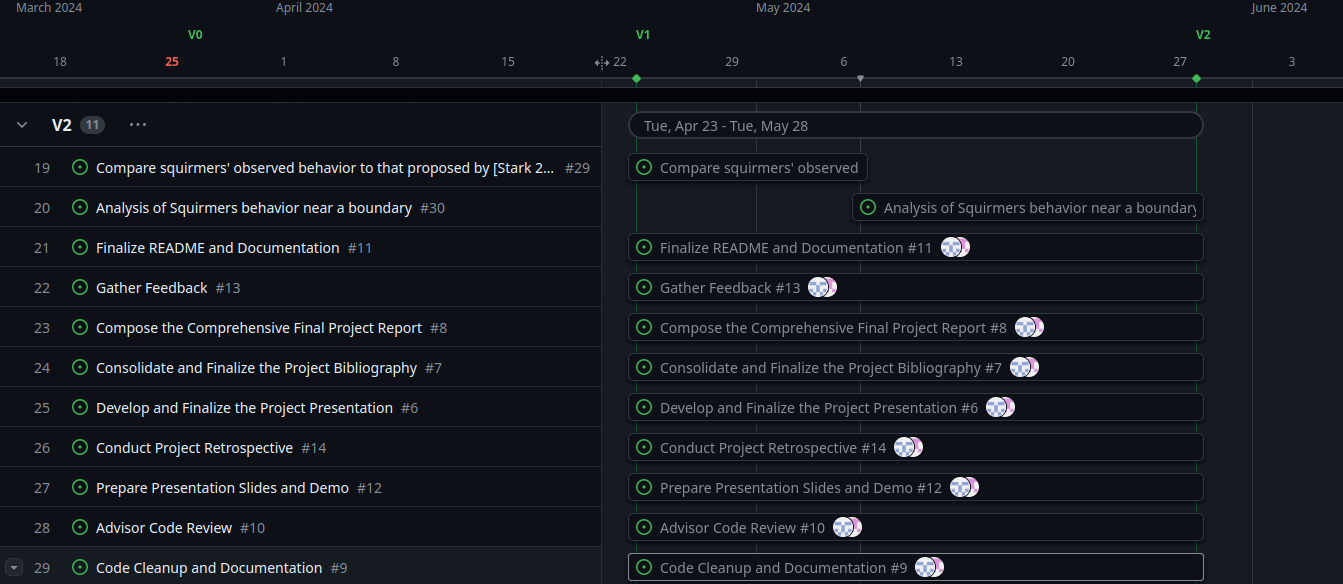
\includegraphics[width=0.9\textwidth]{Presentation/V0/images/roadmapV0_2.png}
\end{center}

\newpage
\section{Velocity field on the squirmer surface}

\textbf{TODO : } ajouter un graphique avec les différents paramètres. Vous 
pouvez utiliser tikz. \\


The time-independent velocity $u$ defined on the surface of the squirmer is given 
in polar coordinates by :

\begin{align*}
   \left\{\begin{array}{rcl}
      u_r(R,\theta) &=& 0 \\
      u_\theta(R,\theta) &=& B_1\mathrm{sin}(\theta)+B_2\mathrm{sin}(\theta)\mathrm{cos}(\theta)
   \end{array}\right.\;
\end{align*}

By setting $\beta=\frac{B_2}{B_1}$, we have :
$$
u_\theta(R,\theta) = B_1(\mathrm{sin}(\theta) + \beta \mathrm{sin}(\theta)\mathrm{cos}(\theta)),
$$
where $\beta$ is the type of the squirmers :
$$\left\{
    \begin{array}{ll}
        \beta = 0 : \text{neutral swimmer}  \\
        \beta < 0 : \mathrm{pusher} \\
        \beta > 0 : \mathrm{puller} \\
    \end{array}
\right.$$
and $B_1$ describes the swimming velocity $u_0 = \frac{2 B_1}{3}$.
\\ Now let us put $u$ in cartesian coordinates :
\begin{align*}
    u &= \begin{pmatrix}
   u_x \\
   u_y
\end{pmatrix}
= \begin{pmatrix}
   \mathrm{cos}(\theta) & -\mathrm{sin}(\theta) \\
   \mathrm{sin}(\theta) & \mathrm{cos}(\theta)
\end{pmatrix}
\begin{pmatrix}
   u_r \\
   u_\theta
\end{pmatrix}, \\
&= B_1 (1 + \beta \mathrm{cos}(\theta))
\begin{pmatrix}
   -\mathrm{sin}^2(\theta) \\
   \mathrm{sin}(\theta)\mathrm{cos}(\theta)
\end{pmatrix}.
\end{align*}
%We have $B_1$ = $\frac{3}{2}u_0$, so :
%$u$ = $\frac{3}{2}u_0 (1 + \beta \mathrm{cos}(\theta))
%\begin{pmatrix}
%   -\mathrm{sin}^2(\theta) \\
%   \mathrm{sin}(\theta)\mathrm{cos}(\theta)
%\end{pmatrix}$

We define $e_r$ the unit vector pointing from the center to the surface 
$$
e_r = \begin{pmatrix}
   \frac{x - x^{cm}}{r}  \\
   \frac{y - y^{cm}}{r} 
\end{pmatrix} = \begin{pmatrix}
   \mathrm{cos}(\theta) \\
   \mathrm{sin}(\theta)
\end{pmatrix}$$ 

and $e$ = 
$\begin{pmatrix}
   \mathrm{cos}(\phi) \\
   \mathrm{sin}(\phi) \end{pmatrix}$ the swimming direction of the squirmer. 
   
   By fixing $\phi$ = 0, one has $e$ = $\begin{pmatrix}
   1 \\
   0 \end{pmatrix}$ and one finds the following expression for the velocity field 
   in cartesian coordinates: 

\begin{align*}
u &= B_1 \left(1+\beta \mathrm{cos}(\theta) \right) \begin{pmatrix}
   -\mathrm{sin}^2(\theta) \\
   \mathrm{sin}(\theta)\mathrm{cos}(\theta)
\end{pmatrix},  \\
&= B_1 \left(1+\beta \mathrm{cos}(\theta) \right) \begin{pmatrix}
   \mathrm{cos}^2(\theta)-1 \\
   \mathrm{sin}(\theta)\mathrm{cos}(\theta)
\end{pmatrix}, \\
&= B_1 \left(1+\beta \begin{pmatrix}
   1 \\
   0 \end{pmatrix}\begin{pmatrix}
   \mathrm{cos}(\theta) \\
   \mathrm{sin}(\theta)
\end{pmatrix}\right) \left[ \left( \begin{pmatrix}
   1 \\
   0 \end{pmatrix}\begin{pmatrix}
   \mathrm{cos}(\theta) \\
   \mathrm{sin}(\theta)
\end{pmatrix}\right) \begin{pmatrix}
   \mathrm{cos}(\theta) \\
   \mathrm{sin}(\theta)
\end{pmatrix} - \begin{pmatrix}
   1 \\
   0 \end{pmatrix}\right], \\
&= B_1(1+\beta (e \cdot e_r)) [(e \cdot e_r)e_r - e]. 
%&= B_1 \left(1+\beta \begin{pmatrix}
%   1 \\
%   0 \end{pmatrix}\begin{pmatrix}
%   \mathrm{cos}(\theta) \\
%   \mathrm{sin}(\theta)
%\end{pmatrix}\right) \left[ \left( \begin{pmatrix}
%   1 \\
%   0 \end{pmatrix}\begin{pmatrix}
%   \mathrm{cos}(\theta) \\
%   \mathrm{sin}(\theta)
%\end{pmatrix}\right) \begin{pmatrix}
%   \mathrm{cos}(\theta) \\
%   \mathrm{sin}(\theta)
%\end{pmatrix} - \begin{pmatrix}
%   1 \\
%   0 \end{pmatrix}\right] \\
% &= B_1 \left(1+\beta \mathrm{cos}(\theta) \right) \begin{pmatrix}
%   \mathrm{cos}^2(\theta)-1 \\
%   \mathrm{sin}(\theta)\mathrm{cos}(\theta)
%\end{pmatrix} \\
%&= B_1 \left(1+\beta \mathrm{cos}(\theta) \right) \begin{pmatrix}
%   -\mathrm{sin}^2(\theta) \\
%   \mathrm{sin}(\theta)\mathrm{cos}(\theta)
%\end{pmatrix} 
\end{align*}

\vspace{0.5 cm}
Thus, $u$ in cartesian coordinates is given by :
\begin{equation*}
\boxed{u_r = B_1(1+\beta (e\cdot e_r)) [(e\cdot e_r)e_r - e].}
   % = \frac{3}{2}u_0\left(1+\beta \mathrm{cos}(\theta) \right) \begin{pmatrix}
   %-\mathrm{sin}^2(\theta) \\
   %\mathrm{sin}(\theta)\mathrm{cos}(\theta)
%\end{pmatrix}}
\end{equation*}

\section{The evolution of the mass center of one squirmers}
The evolution of the mass center $R_i$ = $(X_i, Y_i)$ of one squirmer $i$ is given by :
\begin{center}
$\boxed{\frac{dR_i}{dt}$ = $v_0 p_i - \sum \nabla_{R_{ij}} V_{ij} - \partial_{R_i} V_i + F^{hydro}}$
\end{center}
We have : \begin{itemize}
    \item $v_0$ the particle swimming speed,
    \item $p_i$ = $(\mathrm{cos}(\theta),\mathrm{sin}(\theta))$ orientation,
    \item $F^{hydro}$ the hydrodynamic forces given by Brumley,
    \item $V_{ij}$ and $V_i$, Weeks-Chandler-Andersen potential : repulsive lubrication force avoiding the overlapping of two squirmers. Activated when the distance between two squirmers is small.
\end{itemize} 
\vspace{0,5cm}
$V_{ij}$ = $E_s\left[\left(\frac{2r}{\lvert R_{ij}\rvert}\right)^{12} - \left(\frac{2r}{\lvert R_{ij}\rvert}\right)^6\right]$ and  $V_i$ = $E_s \left[ \left( \frac{r}{\lvert R - R_i \rvert} \right)^{12} - \left( \frac{r}{\lvert R - R_i \rvert} \right) ^6 \right]$ 
\vspace{0,3cm}
\\With : \begin{itemize}
    \item $R_{ij}$ = $\sqrt{D_x^2+D_y^2}$, $\lvert R_{ij} \rvert$ the distance between the centers of two squirmers,
    \item $\lvert R - R_i\rvert$ the distance between the wall and the squirmer center,
    \item $E_s$ a positive constant.
\end{itemize}

\vspace{0,5cm}
We want to calculate : $\nabla_{R_{ij}} V_{ij}$

\begin{align*}
\frac{\partial V_{ij}}{\partial D_x} &= \frac{\partial}{\partial D_x}E_s\left[\left(\frac{2r}{\lvert R_{ij}\rvert}\right)^{12} - \left(\frac{2r}{\lvert R_{ij}\rvert}\right)^6\right] \\
&= E_s \left[\frac{\partial}{\partial D_x}\left(\frac{2r}{\lvert R_{ij}\rvert}\right)^{12} - \frac{\partial}{\partial D_x} \left(\frac{2r}{\lvert R_{ij}\rvert}\right)^6\right] \\
&= E_s \left[ \frac{-12 D_x (2r)^{12}(R_{ij})^{10}}{(R_{ij})^{24}} - \frac{6D_x(2r)^6(R_{ij})^4}{(R_{ij})^12}  \right] \\
&= \frac{-12 E_s}{2r} \left[ \frac{D_x (2r)^{13}}{(R_{ij})^{14}} - \frac{D_x (2r)^{7}}{2(R_{ij})^8}\right] \\
&= \frac{-6 E_s}{2r} \frac{D_x}{R_{ij}} \left[ \frac{2(2r)^{13}}{(R_{ij}^13} - \frac{(2r)^7}{(R_{ij}}\right] \\
&= \frac{-3 E_s}{r} \frac{D_x}{\sqrt{R_{ij}}}\left[ \frac{2(2r)^{13}}{(R_{ij})^13} - \frac{(2r)^7}{(R_{ij})^7} \right]
\end{align*}
Equivalently, we have : 
$\frac{\partial V_{ij}}{\partial D_y}$ = $\frac{-3 E_s}{r} \frac{D_y}{\sqrt{R_{ij}}}\left[ \frac{2(2r)^{13}}{(R_{ij})^13} - \frac{(2r)^7}{(R_{ij})^7} \right]$
\\ Also : 
\begin{equation*}
    \boxed{\nabla_{R_{ij}} V_{ij} = 
    \begin{pmatrix}
        \frac{-3 E_s}{r} \frac{D_x}{\sqrt{R_{ij}}}\left[ \frac{2(2r)^{13}}{(R_{ij})^13} - \frac{(2r)^7}{(R_{ij})^7} \right] \\
        \frac{-3 E_s}{r} \frac{D_y}{\sqrt{R_{ij}}}\left[ \frac{2(2r)^{13}}{(R_{ij})^13} - \frac{(2r)^7}{(R_{ij})^7} \right]
    \end{pmatrix}}
\end{equation*}

\nocite{*}
\bibliographystyle{plain}
\bibliography{/bibliography/biblio}
\end{document}